\documentclass[french]{article}
\usepackage[utf8]{inputenc}
\usepackage[T1]{fontenc}

\usepackage{natbib}
\usepackage[vmargin=3cm,left=4cm,right=4cm]{geometry}

\usepackage{babel}

\usepackage{graphicx}
\usepackage{caption} 
\captionsetup{justification=centering}
\usepackage{subcaption}
% \usepackage{hyperref}
\usepackage[hidelinks]{hyperref}

% ################################
% Package pour incorporer du code
\usepackage{xcolor,colortbl}
\usepackage{listings}

\definecolor{codegreen}{rgb}{0,0.6,0}
\definecolor{codegray}{rgb}{0.5,0.5,0.5}
\definecolor{backcolour}{rgb}{0.95,0.95,0.92}

\lstdefinestyle{mystyle}{
    backgroundcolor=\color{backcolour},   
    commentstyle=\color{codegreen},
    keywordstyle=\color{blue},
    numberstyle=\color{codegray},
    stringstyle=\color{orange},
    basicstyle=\ttfamily\small, % \footnotesize,
    breakatwhitespace=false,         
    breaklines=true,                 
    captionpos=b,                    
    keepspaces=true,                 
    numbers=left,                    
    numbersep=10pt,                  
    showspaces=false,                
    showstringspaces=false,
    showtabs=false,
    literate=
  {²}{{\textsuperscript{2}}}1
  {⁴}{{\textsuperscript{4}}}1
  {⁶}{{\textsuperscript{6}}}1
  {⁸}{{\textsuperscript{8}}}1
  {€}{{\euro{}}}1
  {é}{{\'e}}1
  {è}{{\`{e}}}1
  {ê}{{\^{e}}}1
  {ë}{{\¨{e}}}1
  {É}{{\'{E}}}1
  {Ê}{{\^{E}}}1
  {û}{{\^{u}}}1
  {ù}{{\`{u}}}1
  {â}{{\^{a}}}1
  {à}{{\`{a}}}1
  {á}{{\'{a}}}1
  {ã}{{\~{a}}}1
  {Á}{{\'{A}}}1
  {Â}{{\^{A}}}1
  {Ã}{{\~{A}}}1
  {ç}{{\c{c}}}1
  {Ç}{{\c{C}}}1
  {õ}{{\~{o}}}1
  {ó}{{\'{o}}}1
  {ô}{{\^{o}}}1
  {Õ}{{\~{O}}}1
  {Ó}{{\'{O}}}1
  {Ô}{{\^{O}}}1
  {î}{{\^{i}}}1
  {Î}{{\^{I}}}1
  {í}{{\'{i}}}1
  {Í}{{\~{Í}}}1
}

\lstset{style=mystyle}

%##################################

% MLD
%##################################

\usepackage[normalem]{ulem}
\newenvironment{mld}
  {\par\begin{minipage}{\linewidth}\begin{tabular}{rp{0.7\linewidth}}}
  {\end{tabular}\end{minipage}\par}
\newcommand{\relat}[1]{\textsc{#1}}
\newcommand{\attr}[1]{\emph{#1}}
\newcommand{\prim}[1]{\uline{#1}}
\newcommand{\foreign}[1]{\#\textsl{#1}}

%####################################

\begin{document}

%###############################################
\begin{titlepage}

\newcommand{\HRule}{\rule{\linewidth}{0.5mm}} % Defines a new command for the horizontal lines, change thickness here

\center % Center everything on the page
 
%----------------------------------------------------------------------------------------
%	Section Titre
%----------------------------------------------------------------------------------------
\HRule \\[0.4cm]
\vspace{1cm}
{ \huge \bfseries Projet de Gestion de Stock}\\ % Title of your document
\vspace{1cm}
\HRule \\[1cm]
 
%----------------------------------------------------------------------------------------
%	Section auteur
%----------------------------------------------------------------------------------------
\vspace{1cm}

\Large \today

\vspace{3cm}

\begin{minipage}{0.4\textwidth}
\begin{center}
\Large \textbf{Auteurs :}\\
\vspace{0.5cm}
Sylvia \textsc{Penfeunteun} \\
Hervé \textsc{Poirier}\\
Thierry \textsc{Adam}\\
Nathan \textsc{Faudeil}\\
Fabio \textsc{Cassiano}
\end{center}
\end{minipage}

\vspace{5cm}

\begin{figure}[!ht]
    %\hspace*{-0.5cm}
	
\includegraphics[height=0.1\columnwidth]{Image/logo/logo_simplon.png}
	\hspace*{0.5cm}
	
\includegraphics[height=0.12\columnwidth]{Image/logo/logo_Isen.png}
	\hspace*{0.5cm}
	
\includegraphics[height=0.1\columnwidth]{Image/logo/logo_microsoft.jpg}
\end{figure}

\vfill

\end{titlepage}

\newpage

\tableofcontents

\newpage

\section{Règles de gestion}
\begin{itemize}
    \item Une usine fabrique plusieurs références et une référence peut être construite par plusieurs usines.
    \item Une facture est destinée à un seul client, un client peut avoir plusieurs facutres.
    \item Une facture peut avoir plusieurs produits et les produits apparaissent sur plusieurs factures.

\end{itemize}

\section{Dictionnaire des données}

A partir des règles de gestion précédentes, ainsi que les différentes informations de l'entreprise, il nous a été possible de mettre en place le dictionnaire de données. Dans ce dictionnaire on retrouve :
\begin{itemize}
    \item le libellé de chaque élément de la base
    \item la description correspondant à chaque libellé
    \item le type de donnée : Alphabétique (A), Numérique (N), Alphanumérique (AN)
    \item la taille possible de chaque élément
    \item une remarque, si nécessaire.
\end{itemize}

\begin{table}[!htbp]
\begin{tabular}{|lcccl|}
\hline
\multicolumn{1}{|l|}{\textbf{Libellé}}     & \multicolumn{1}{c|}{\textbf{Description}}        & \multicolumn{1}{c|}{\textbf{Type}} & \multicolumn{1}{c|}{\textbf{Taille}} & \multicolumn{1}{c|}{\textbf{Remarque}}          \\ \hline
	
\multicolumn{5}{|l|}{\textbf{Usines}}                                                                                                                                                               \\ \hline
\multicolumn{1}{|l|}{id\_usine}            & \multicolumn{1}{c|}{Idetifiant de l'usine}       & \multicolumn{1}{c|}{N}             & \multicolumn{1}{c|}{11}              &                                                 \\ \hline
\multicolumn{1}{|l|}{nom\_usine}           & \multicolumn{1}{c|}{Nom de l'usine}              & \multicolumn{1}{c|}{A}             & \multicolumn{1}{c|}{30}              &                                                 \\ \hline
\multicolumn{1}{|l|}{adresse\_usine}       & \multicolumn{1}{c|}{Adresse de l'usine}          & \multicolumn{1}{c|}{A}             & \multicolumn{1}{c|}{50}              &                                                 \\ \hline
\multicolumn{1}{|l|}{ville\_usine}         & \multicolumn{1}{c|}{Ville de l'usine}            & \multicolumn{1}{c|}{A}             & \multicolumn{1}{c|}{30}              &                                                 \\ \hline
\multicolumn{5}{|l|}{\textbf{Clients}}                                                                                                                                                              \\ \hline
\multicolumn{1}{|l|}{id\_client}           & \multicolumn{1}{c|}{Identifiant client}          & \multicolumn{1}{c|}{N}             & \multicolumn{1}{c|}{11}              &                                                 \\ \hline
\multicolumn{1}{|l|}{nom\_client}          & \multicolumn{1}{c|}{Nom du client}               & \multicolumn{1}{c|}{A}             & \multicolumn{1}{c|}{50}              &                                                 \\ \hline
\multicolumn{1}{|l|}{adresse\_client}      & \multicolumn{1}{c|}{Adresse du client}           & \multicolumn{1}{c|}{A}             & \multicolumn{1}{c|}{50}              &                                                 \\ \hline
\multicolumn{1}{|l|}{ville\_client}        & \multicolumn{1}{c|}{Ville du client}             & \multicolumn{1}{c|}{A}             & \multicolumn{1}{c|}{30}              &                                                 \\ \hline
\multicolumn{1}{|l|}{pays\_client}         & \multicolumn{1}{c|}{Pays du client}              & \multicolumn{1}{c|}{A}             & \multicolumn{1}{c|}{20}              & \multicolumn{1}{c|}{}                           \\ \hline
\multicolumn{5}{|l|}{\textbf{Types}}                                                                                                                                                                \\ \hline
\multicolumn{1}{|l|}{id\_type}             & \multicolumn{1}{c|}{Identifiant type}            & \multicolumn{1}{c|}{N}             & \multicolumn{1}{c|}{11}              &                                                 \\ \hline
\multicolumn{1}{|l|}{nom\_type}            & \multicolumn{1}{c|}{Nom du types}                & \multicolumn{1}{c|}{A}             & \multicolumn{1}{c|}{30}              &                                                 \\ \hline
\multicolumn{5}{|l|}{\textbf{Produits}}                                                                                                                                                             \\ \hline
\multicolumn{1}{|l|}{id\_produit}          & \multicolumn{1}{c|}{Identifiant du produit}      & \multicolumn{1}{c|}{N}             & \multicolumn{1}{c|}{11}              &                                                 \\ \hline
\multicolumn{1}{|l|}{ref\_produit}         & \multicolumn{1}{c|}{Référence du produit}        & \multicolumn{1}{c|}{AN}            & \multicolumn{1}{c|}{15}              &                                                 \\ \hline
\multicolumn{1}{|l|}{nom\_produit}         & \multicolumn{1}{c|}{Nom du produit}              & \multicolumn{1}{c|}{A}             & \multicolumn{1}{c|}{50}              &                                                 \\ \hline
\multicolumn{1}{|l|}{description\_produit} & \multicolumn{1}{c|}{Description du produit}      & \multicolumn{1}{c|}{A}             & \multicolumn{1}{c|}{50}              &                                                 \\ \hline
\multicolumn{1}{|l|}{statut\_produit}      & \multicolumn{1}{c|}{Statut du produit}           & \multicolumn{1}{c|}{N}             & \multicolumn{1}{l|}{}                & \multicolumn{1}{c|}{booleen (abandonné ou pas)} \\ \hline
\multicolumn{5}{|l|}{\textbf{Commander}}                                                                                                                                                            \\ \hline
\multicolumn{1}{|l|}{id\_commander}        & \multicolumn{1}{c|}{Identifiant de la commandes} & \multicolumn{1}{c|}{N}             & \multicolumn{1}{c|}{11}              &                                                 \\ \hline
\multicolumn{1}{|l|}{quantite\_commander}  & \multicolumn{1}{c|}{Quantité de la commande}     & \multicolumn{1}{c|}{N}             & \multicolumn{1}{c|}{11}              &                                                 \\ \hline
\multicolumn{5}{|l|}{\textbf{Facture}}                                                                                                                                                              \\ \hline
\multicolumn{1}{|l|}{id\_facture}          & \multicolumn{1}{c|}{Identifiant de la facture}   & \multicolumn{1}{c|}{N}             & \multicolumn{1}{l|}{}                &                                                 \\ \hline
\multicolumn{1}{|l|}{numero\_facture}      & \multicolumn{1}{c|}{Numero de la facture}        & \multicolumn{1}{c|}{AN}            & \multicolumn{1}{l|}{}                &                                                 \\ \hline
\multicolumn{5}{|l|}{\textbf{Calendrier}}                                                                                                                                                           \\ \hline
\multicolumn{1}{|l|}{date\_calendrier}     & \multicolumn{1}{c|}{Date du calendrier}          & \multicolumn{1}{c|}{N}             & \multicolumn{1}{c|}{10}              & \multicolumn{1}{c|}{date, clé primaire}         \\ \hline
\end{tabular}
\caption{Dictionnaire des données correspondant système de facturation d'IKEO}
\end{table}

\section{Dépendances fonctionnelles}

\begin{itemize}
    \item \textbf{id\_client}? nom\_client, adresse\_client, ville\_client, pays\_client, id\_types
    \item \textbf{id\_facture}? numero\_facture, date\_calendrier, id\_client
    \item \textbf{id\_produit}? reference\_produit, nom\_produit, description\_produit, statut\_produit
    \item \textbf{id\_usine}? nom\_usine, adresse\_usine, ville\_usine
    \item \textbf{id\_type}? nom\_types
\end{itemize}

\section{Schéma entité-association}

\begin{figure}[!htbp]
    \centering
    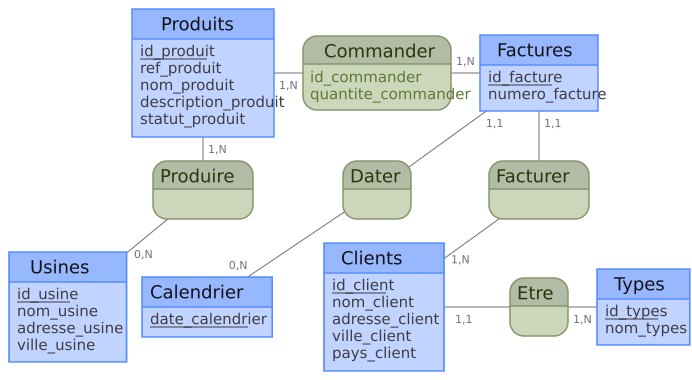
\includegraphics[width=\textwidth]{Rapport/Image/schema_EA.png}
    \caption{Schéma entité-association pour le projet de facturation de l'entreprise IKEO}
    \label{fig:schema_bdd}
\end{figure}
    
\section{MLD}


\begin{mld}
  \textbf{Produits} & (\prim{id\_produit}, \attr{ref\_produit}, \attr{nom\_produit}, \attr{description\_produit}, \attr{statut\_produit})\\
  \textbf{Commander} & (\foreign{\prim{id\_produit}}, \foreign{\prim{id\_facture}}, \attr{id\_commander}, \attr{quantite\_commander})\\
  \textbf{Factures} & (\prim{id\_facture}, \attr{numero\_facture}, \foreign{date\_calendrier}, \foreign{id\_client})\\
  \textbf{Produire} & (\foreign{\prim{id\_usine}}, \foreign{\prim{id\_produit}})\\
  \textbf{Usines} & (\prim{id\_usine}, \attr{nom\_usine}, \attr{adresse\_usine}, \attr{ville\_usine})\\
  \textbf{Calendrier} & (\prim{date\_calendrier})\\
  \textbf{Clients} & (\prim{id\_client}, \attr{nom\_client}, \attr{adresse\_client}, \attr{ville\_client}, \attr{pays\_client}, \foreign{id\_types})\\
  \textbf{Types} & (\prim{id\_types}, \attr{nom\_types})\\
\end{mld}

\newpage
\section{Schéma de la base créer}

\begin{figure}[!htbp]
    \centering
    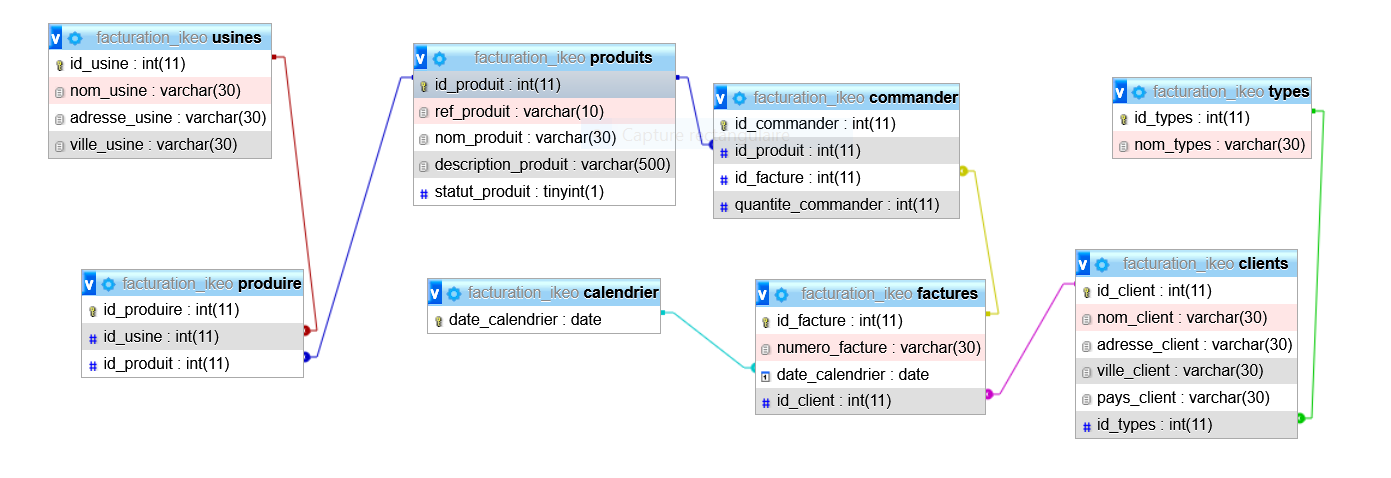
\includegraphics[width=\textwidth]{Rapport/Image/schema_bdd.PNG}
    \caption{Schéma de la base de données créer sur MySQL.}
    \label{fig:schema_bdd}
\end{figure}


\section{requête SQL}

\begin{lstlisting}[language=sql]
-- • Afficher les noms et descriptions de tous les produits:

SELECT nom_produit, description_produit FROM produits 

-- • Afficher tous les meubles qui sont abandonnés:

SELECT nom_produit FROM produits WHERE statut_produit='0' 

-- • Effacer le Bo Meuble de brest:

DELETE FROM clients WHERE nom_client='Bo Meuble' AND ville_client ='Brest' 
DELETE FROM clients WHERE nom_client='Bo Meuble' AND adresse_client='Rue Jean Jaurès' AND ville_client ='Brest' AND pays_client='France'

-- • Il y a une erreur sur le nom du meuble Apfelgluk, il faut le réécrire Apfelgluck:

UPDATE produits SET nom_produit = 'Apfelgluck' WHERE ref_produit='OANT12'

-- • Ajouter un nouveau client : Tout à la maison, Place Terreaux, Lyon:

-- Version 1 :
INSERT INTO clients (id_types, nom_client, adresse_client, ville_client, pays_client) VALUES ('1', 'Tout à la maison', 'Place Terreaux', 'Lyon', 'France')

-- Version 2:
INSERT INTO clients (id_types, nom_client, adresse_client, ville_client, pays_client) VALUES ((SELECT id_types FROM types WHERE nom_types='Magasin'), 'Tout à la maison', 'Place Terreaux', 'Lyon', 'France')


-- • Ajouter une nouvelle facture pour le Tout à la maison de Lyon , enregistrée le 28/08/2018, à 18h: (La commande est composé de 18 Naess)     

INSERT INTO calendrier (date_calendrier) VALUES ('2018-08-28 18:00:00')
INSERT INTO factures (numero_facture, date_calendrier, id_client) VALUES ('MSQ298', '2018-08-28 18:00:00', (SELECT id_client FROM clients WHERE nom_client = "Tout à la maison" AND ville_client = "Lyon"))
INSERT INTO commander (id_produit, id_facture, quantite_commander) VALUES ((SELECT id_produit FROM produits WHERE nom_produit = "Naess"), (SELECT id_facture FROM factures WHERE numero_facture = 'MSQ297'), 18)



-- • Retrouver tous les meubles achetés par le Bo Meuble de Paris: (clients, factures, calendrier)
SELECT nom_client,ville_client, id_facture, nom_produit, ref_produit, quantite_commander FROM clients NATURAL JOIN factures NATURAL JOIN commander NATURAL JOIN produits WHERE nom_client='Bo Meuble' AND ville_client='Paris'
SELECT nom_produit, quantite_commander FROM produits NATURAL JOIN commander NATURAL JOIN factures WHERE id_client= '1'

-- • Retrouver toutes les factures enregistrées depuis le 1er juillet 2018:

SELECT * FROM facturation_ikeo.calendrier WHERE date_calendrier > '2018-07-01 00:00:00'
\end{lstlisting}

\end{document}
